\documentclass{article}
\usepackage[utf8]{inputenc}

\title{Analiza wpływu gospodarczego na inne aspekty życia.}
\usepackage{polski}
\usepackage[utf8]{inputenc}
\usepackage{caption}
\usepackage{natbib}
\usepackage{graphicx}

\begin{document}

\maketitle

\section{Problem}
Projekt ma na celu analizę wpływu gospodarczego (mierzonego miernikiem PKB) na dane z różnych sfer oraz aspektów życią.
Wstępna obróbka danych została wykonana w Scali oraz Sparku - scalenie powiązanych ze sobą tabel, wstepna filtracja oraz transformacja do
macierzy umożliwiającej łatwiejszą dalszą analizę. W kolejnym etapie analizy, wykorzystany został Python wraz z Jupyter Noteboo, który zapewnia
interaktywne wykonanie kodu, oraz standardowe biblioteki takie jak: Pandas, NumPy, Matplotlib.


\section{Linki}

Dane zawierają 195 wskaźników z 30 różnych dziedzin dla 159 państw.

https://www.kaggle.com/worldbank/world-development

https://www.kaggle.com/kumarajarshi/life-expectancy-who/data


\clearpage


\section{Spotkania}

\begin{itemize}
  \item 02.03.2020
  
   Zrealizowane zadania
    \begin{itemize}
        \item pobranie danych
        \item zapoznanie się z danymi
    \end{itemize}
    
    Zadania na następne spotkanie:
    \begin{itemize}
        \item wstępna analiza danych z wykorzystaniem metody PCA
        \item prezentacja rozkładów danych, histogramy
    \end{itemize}

  \item 16.03.2020
  
    Zrealizowane zadania:
    \begin{itemize}
        \item analiza danych z wykorzystaniem metody PCA
        \item prezentacja histogramów dla poszczególnych danych
        \item przeniesiono dokumentację do formatu Latex
    \end{itemize}
    
    Zadania na następne spotkanie:
    \begin{itemize}
        \item "Proszę zanalizować oprócz średniej długości życia również pozostałe elementy: rozmiar ubóstwa i
nierówności majątkowe"
    \end{itemize}
  
  \item 23.03.2020
  
    Zrealizowane zadania:
    \begin{itemize}
        \item
    \end{itemize}
    
    Zadania na następne spotkanie:
    \begin{itemize}
        \item
    \end{itemize}
  
  \item 30.03.2020
  
    Zrealizowane zadania:
    \begin{itemize}
        \item
    \end{itemize}
    
    Zadania na następne spotkanie:
    \begin{itemize}
        \item
    \end{itemize}
  
\end{itemize}

\clearpage
\section{Szczegółowe omówienie zrelizowanych zadań}

\subsection{02.03.2020}
  
  ---
  
\subsection{16.03.2020} 
  
\subsubsection{Wstępne porównanie wartości parametrów PKB oraz długości życia.}

Na wstępie przeanalizowano średnią długość życia oraz średnią wartość GDP dla każdego z państw.
Wartość GDP oraz średnia długość życia pełnią role etykiet.
Wyniki przedstawiono przy użyciu histogramów. Zdecydowano się na wybór wartości średnich wyliczonych dla każdego z państw na przestrzeni 15 lat,
gdyż prezentacja dla poszczególnych lat mogłaby skutkować większą ilością rekordów nie zawierających żadnych danych (z powodu braków w danych).
Wyniki zaprezentowanano na rysunku \ref{fig:1_1_GDP_vs_LE}.

\begin{figure}[h!]
\begin{center}
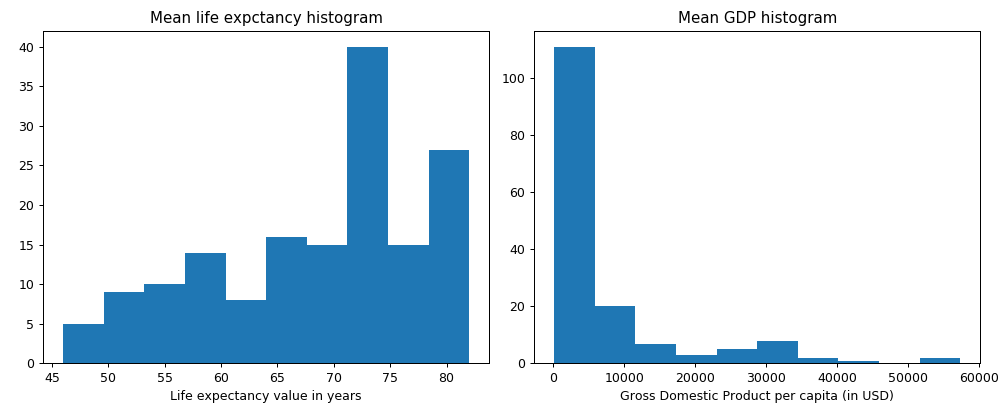
\includegraphics[width=5 in]{Pictures/1_GDP_vs_LE.png}
\end{center}
\captionsetup{justification=centering}
\caption{Porównanie rozkładu danych PKB i długości życia.}
\label{fig:1_1_GDP_vs_LE}
\end{figure}
  
Trudno jest wysunąć wnioski na temat powiązania obu wyników, gdyż wartości minimalne oraz maksymalne prezentowane przez histogram przedstawiający wartości GDP są są bardzo rozbieżne, a większość z nich
znajduje się w pierwszym przedziale. Dane GDP wykorzystane do takiej analizy porównawczej są zbyt ogólne.
 
\clearpage
Zdecydowano się na obserwację zmian dla każdego z tych parametrów na przestrzeni lat 2005 - 2015. Wyniki przedstawiono również przy użyciu histogramów.

\begin{figure}[h!]
\begin{center}
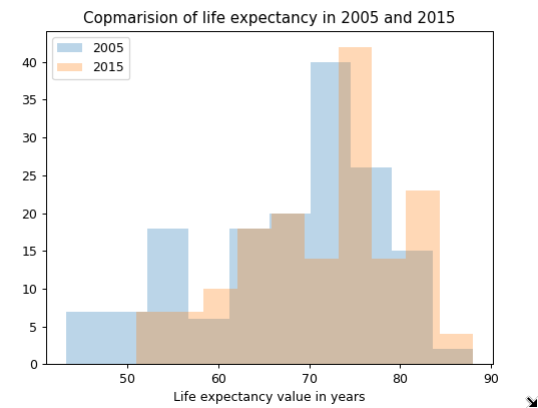
\includegraphics[width=3 in]{Pictures/2_LE_2005_vs_2015.png}
\end{center}
\captionsetup{justification=centering}
\caption{Porównanie rozkładu wartości długości życia w latach 2005 i 2015.}
\label{fig:2_LE_2005_2015}
\end{figure}

Na histogramie \ref{fig:2_LE_2005_2015} zaobserwowano ogólny wzrost wartości długości życia.
Może to być skutkiem ogólnej poprawy jakości życia oraz rozwoju gospodarczego państw.

% \clearpage

\begin{figure}[h!]
\begin{center}
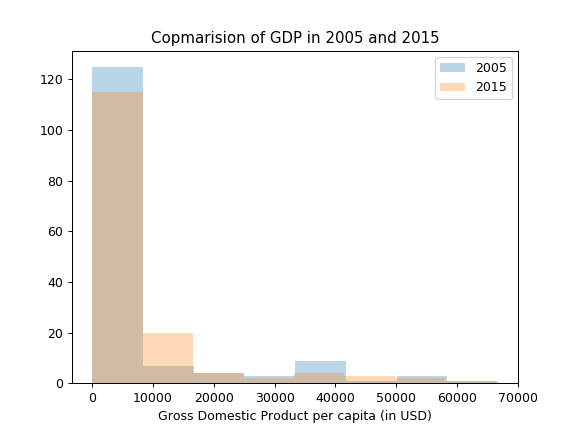
\includegraphics[width=3 in]{Pictures/3_GDP_2005_vs_2015.png}
\end{center}
\captionsetup{justification=centering}
\caption{Porównanie rozkładu wartości PKB w latach 2005 i 2015.}
\label{fig:3_PKB_2005_2015}
\end{figure}

Zmiany dotyczące wskaźnika GDP są w momencie takiej analizy widoczne.
Pokazują one ogólną poprawę współczynnika GDP wśród państw.

\clearpage
\subsubsection{Wstępna analiza PCA}

Następnie wykonano analizę PCA dla danych.

TODO opisać wykorzystaną metodę interpolacji

Pierwszą próbę podjęto wykorzystując dane o 185 cechach.
Na rysunku \ref{fig:4_PCA_full} przedstawiono otrzymane punkty na płaszczyźnie dwu wymiarowej.

\begin{figure}[h!]
\begin{center}
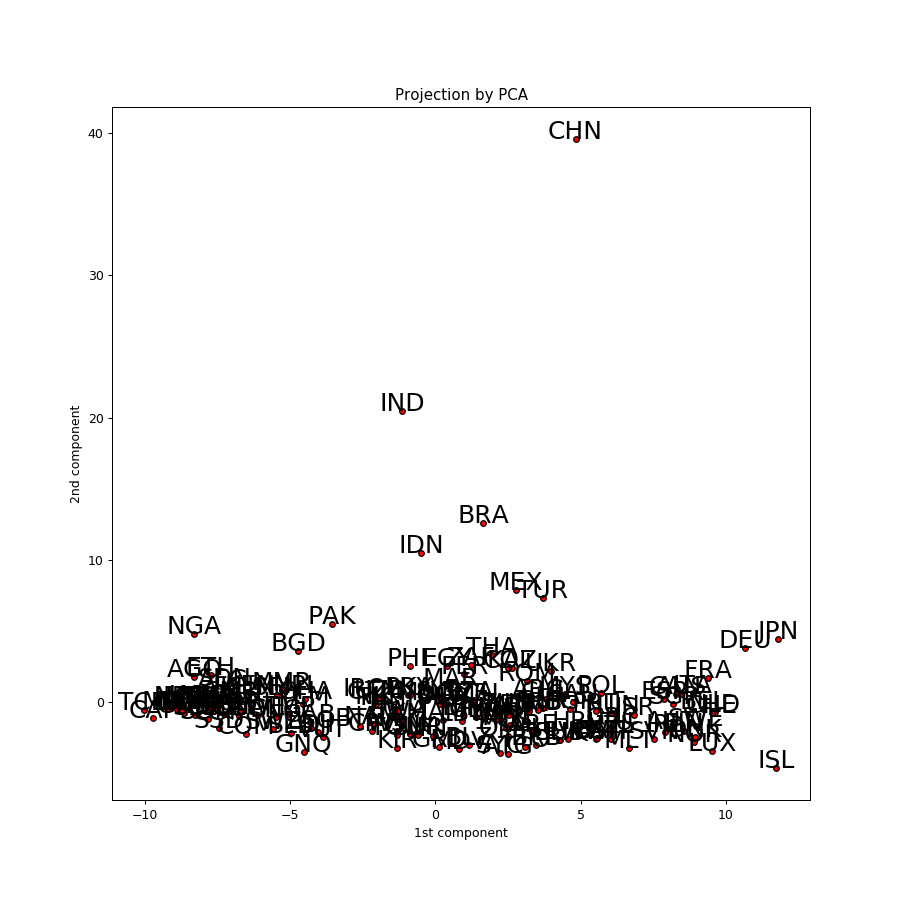
\includegraphics[width=5 in]{Pictures/4_PCA_full.png}
\end{center}
\captionsetup{justification=centering}
\caption{Analiza PCA dla pełnych danych.}
\label{fig:4_PCA_full}
\end{figure}

Procent wariancji wyjaśniony przez dwa wiądące wskaźniki wyniósł 0,28.
Jest to dość niska wartość.

Państwa wysunięte na lewą stronę prezentowanej płaszczyzny to państwa o wysokim poziomie współczynnika
urodzeń na 1000 mieszkańców, z dużym odsetkiem ludności mieszkającej na wsi oraz ze sporym odsetkiem ludzi żyjących za mniej niż 3.10\$ na dzień. Państwa znajdujące się w tym obszarze to państwa słabo rozwinięte, takie jak Nigeria, Madagaskar, Malawi.
Państwa wysunięte na prawą stronę to państwa zurbanizowane, a więc takie posiadające dostęp do paliwa
stałego, elektryczności oraz posiadające spory odsetek ludności mieszkającej w miastach. Posiadają one również dużą długość życia oraz wysoki współczynnik PKB. Są to na przykład Chiny, Japonia, Niemcy, Islandia.

Współczynniki odpowiadające za położenie w górnej lub dolnej części są niejednoznaczne i trudne do interpretacji.

W zaprezentowanych danych pojawiało się po kilka cech z danej przestrzeni/sektora życia. Zdecydowano się na analizę danych wybierając losowo po
jednej cesze z danego sektora.
Otrzymano tym samym dane 32 wymiarowe. Wyniki przedstawiono na rysnuiku \ref{fig:5_PCA_partial}:

\begin{figure}[h!]
\begin{center}
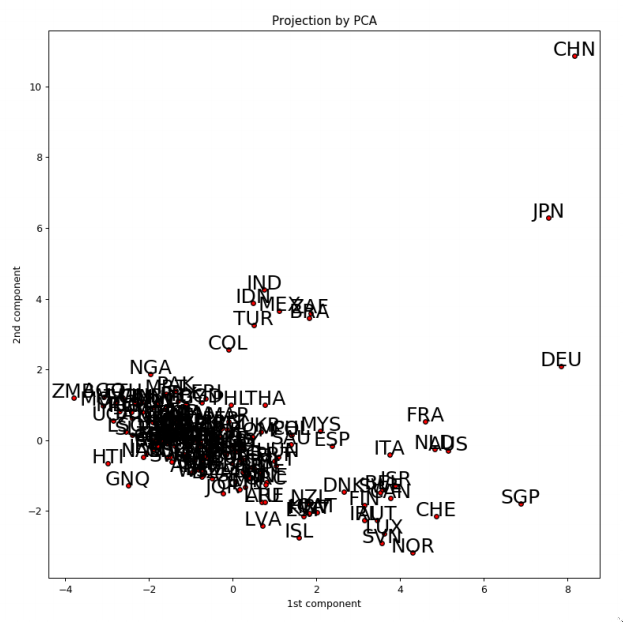
\includegraphics[width=5 in]{Pictures/5_PCA_parital.png}
\end{center}
\captionsetup{justification=centering}
\caption{Analiza PCA dla losowo wybranych danych z każdego sektora.}
\label{fig:5_PCA_partial}
\end{figure}


Procent wariancji wyjaśniony przez dwa wiodące wskaźniki wyniósł 0,31.
Jest to dość niska wartość.

Po prawej stronie płaszczyzny są umieszczane państwa, które przeznaczają dużo kosztów na badania o
charakterze rozwojowym, posiadają wysoki współczynnik GDP oraz posiadają wysokie wydatki na fundusz zdrowotny.
Są to państwa wysoko rozwinięte takie jak Chiny, Niemcy, Singapur czy Japonia.
Po przeciwnej stronie są państwa posiadające duży współczynnik urodzeń, wysoki współczynnik inflacji
czy wysoki współczynnik mieszkańców żyjący za mniej niż 3,10\$ dziennie.
W tej grupie znalazły się znowu państwa biedne oraz słabo rozwinięte.
Współczynniki odpowiadające za położenie w górnej lub dolnej części tak samo są niejednoznaczne i trudne do interpretacji.

  \clearpage

\subsection{23.03.2020}

\subsubsection{Analiza współczynniku bezrobocia.}

Przeprowadzono analizę współczynnika dla poszczególnych regionów świata w latach 2011-2014. Wyniki przedstawiono na rysunku \ref{fig:7_world_unemployment_regions}.

\begin{figure}[h!]
\begin{center}
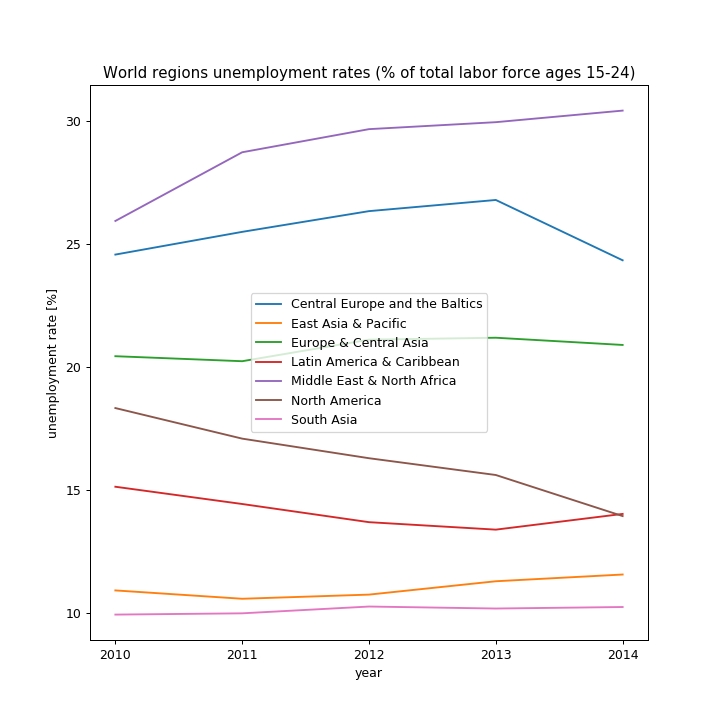
\includegraphics[width=5 in]{Pictures/7_unemployment_world_regions.png}
\end{center}
\captionsetup{justification=centering}
\caption{Współczynnik bezrobocia w poszczególnych regionach świata w grupie 15-24 lata w latach 2011-2014.}
\label{fig:7_world_unemployment_regions}
\end{figure}

Trudno jest wyciągnąć wnioski łączące oba te rysunki, gdyż rysnek \ref{fig:7_world_unemployment_regions} uwzględniają one liczby ludności zamieszkującej dane regiony świata. 

\clearpage
Przeprowadzono w związku z tym analizę obejmującą poszczególne państwa. Wybrano losowo 68 państw oraz następnie przeanalizowano dla nich zmiany współczynnika PKB oraz zmiany współczynnika bezrobocia w grupie 15-24 lat w latach 2011-2014.

\begin{figure}[h!]
\begin{center}
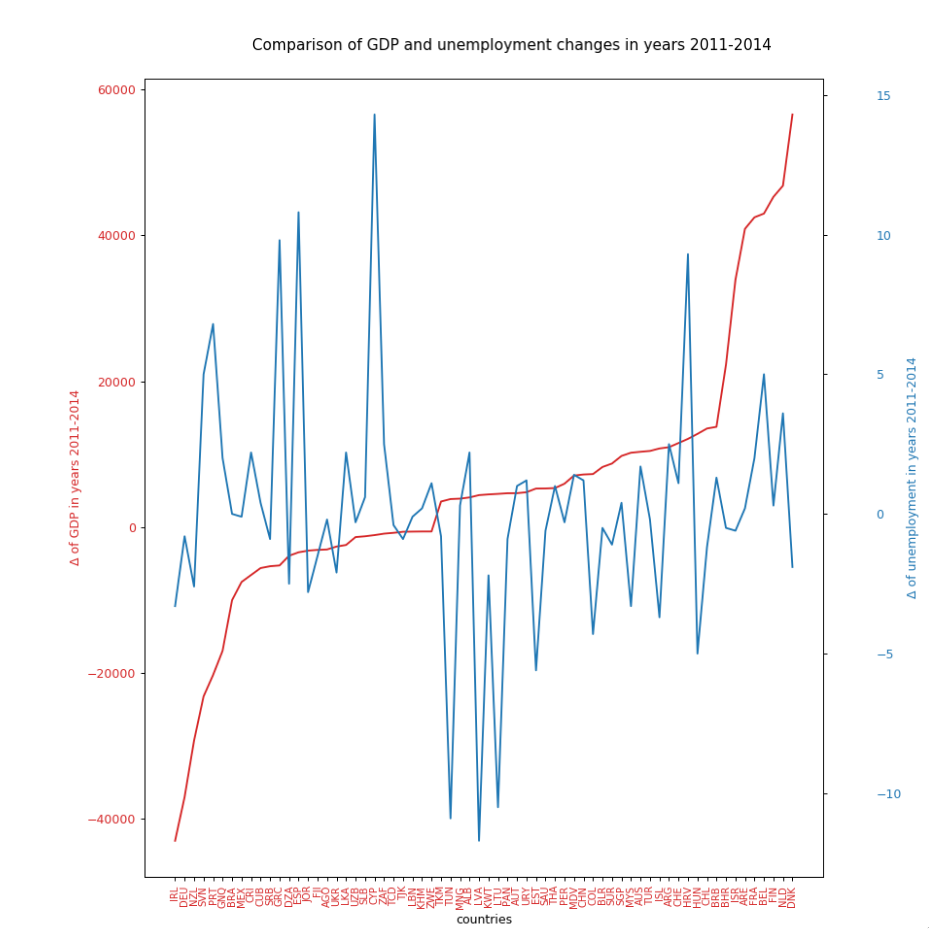
\includegraphics[width=5 in]{Pictures/8_gdp_vs_unemployment.png}
\end{center}
\captionsetup{justification=centering}
\caption{Porównanie zależności zmian współczynnika bezrobocia a zmian współczynnika PKB w latach 2011-2014.}
\label{fig:8_unemployment_vs_gdp}
\end{figure}

Pomimo, że dane biorą pod uwagę zmiany na przestrzeni tylko 4 latach, co jest dość krótkim okresem, obserwujemy widoczną zależność pomiędzy dwoma analizowanymi współczynnikami. Państwa notujące w tych latach spadek współczynnika PKB odnotowują mniejsze, bądź większe wzrosty bezrobocia. Natomiast państwa notujące wzrost współczynnika PKB na przestrzeni analizowanych lat odnotowują spadek bezrobocia. W danych pojawiają się pewne niespójności oraz wyjątki. Jest to skutek dostępnych danych, które zostały zebrane w krótkim odcinku czasu.

Następnie przeanalizowano jaki odsetek bezrobotnych stanowią ludzie z wykształceniem podstawowym, średnim oraz wyższym. 
Do analizy wybrano 20 krajów z najniższym PKB oraz 20 krajów z najwyższym współczynnikiem.

\begin{figure}[h!]
\begin{center}
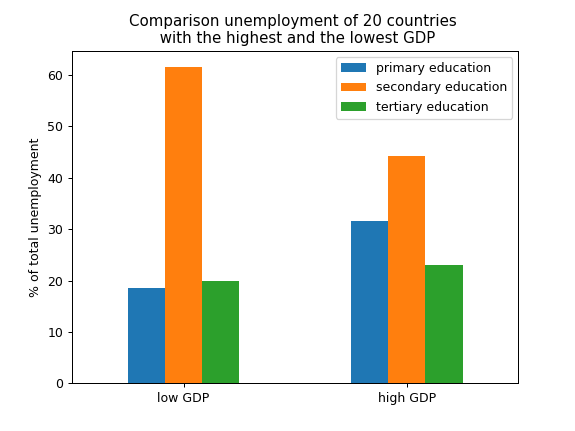
\includegraphics[width=5 in]{Pictures/9_unemployment_and_degree.png}
\end{center}
\captionsetup{justification=centering}
\caption{Porównanie bezrobotnych z grupy najmniej}
\label{fig:9_unemployment_vs_education}
\end{figure}

Wartości prezentowane na wykresie \ref{fig:9_unemployment_vs_education} przedstawiają jaki odsetek wszystkich bezrobotnych stanowi dana grupa. Wartości te zostały te wyliczone jako średnia wartości każdego z 20 państw w związku z tym mogą się one nie sumować dokładnie do 100\%. Prezentowane wyniki są dość ciekawe. Obserwujemy tutaj widoczną różnicę pomiędzy krajami o niskim oraz wysokim PKB. Dla grupy o niskim współczynniku PKB znacznie dominującą grupą jest grupa ludzi posiadających wykształcenie średnie. Dla państw o wysokim PKB wartości te nie są aż tak rozbieżne. 

\subsubsection{Analiza współczynnika ubóstwa.}

\clearpage

\subsection{30.03.2020}

\end{document}
